\chapter*{Prostor obrazových signálů}
%
V této kapitole bude podán přehled základních teoretických nástrojů, které jsou potřebné pro kvalifikované zvládnutí problematiky digitálního zpracování obrazu.
Čtenáře zde prosíme o určitou dávku trpělivosti. Bez pochopení skutečností uvedených v této kapitole se zpracováním obrazu nelze seriózně zabývat.
Protože každý optický obraz je signálem, budeme v této kapitole poněkud obecnější a místo o obrazu nebo obrazovém signálu budeme často obecně hovořit pouze o signálu.
Závěry, které zde uvedeme, platí pro jakékoli signály, a tedy i pro signály obrazové. Obrazové signály jsou zpravidla dvojrozměrné.
S ohledem na tuto skutečnost budeme vztahy, které budou později prakticky využívány, ihned formulovat také v jejich dvojrozměrných variantách.

\section*{Prostor signálů}

Předpokládáme, že signál je definován nad jistou podmnožinou (označme ji $\Omega$) $m$-rozměrného euklidovského prostoru $E^m$.
Touto podmnožinou může být nějaká ohraničená nebo neohraničená souvislá oblast v $E^m$, množina jednotlivých bodů z $E^m$, ale také celý prostor $E^m$.
Jako matematickou reprezentaci signálu zvolíme funkci $f:\Omega \rightarrow \gamma$, kde $\gamma$ je obor hodnot signálu.
Množina $\gamma$ může být např. množinou celých nebo reálných čísel (obrazy ve stupních šedi), množinou komplexních čísel
(obrazy vznikající některými transformacemi), množinou vektorů o třech složkách (v barevných obrazech bývá často barva každého bodu popsána trojicí $R$, $G$, $B$, jejíž jednotlivé členy udávají intenzitu červené, zelené a modré barevné složky) nebo podmnožinou některé z uvedených množin. O signálu $f$ řekneme, že je $m$-rozměrným signálem.
Množinu funkcí realizujících zobrazení $\Omega \rightarrow \gamma$, kde $\gamma$ nazveme $m$-rozměrným signálovým prostorem $\mathscr{S}$. Je tedy $\mathscr{S} = { f | f:\Omega \rightarrow \gamma }$.
Úvahy provedené v této kapitole se budou týkat zejména signálů reálných a komplexních.
Doplňující informace, které se týkají signálů reprezentovaných celými čísly a vektory, uvedeme na vhodném místě později.

\subsection*{Linearita prostoru signálů}
%
Při zpracování signálů dosti často předpokládáme, že pro signály platí princip superpozice.
Matematickým vyjádřením této představy je, že signálový prostor předpokládáme lineární.
Zopakujme, že v lineárním prostoru je definována operace sčítání prvků a násobení prvku konstantou (konstantou může být reálné nebo komplexní číslo).
Připomeňme dále, že v lineárním prostoru existuje nulový prvek a ke každému prvku existuje prvek opačný.

Uvažujme nejprve prostor jednorozměrných diskrétních signálů (označme jej $\mathscr{S}$), kde definičním oborem $\Omega$ je množina $M$ bodů.
Každý bod je popsán svým indexem $m$. Bez újmy na obecnosti lze předpokládat, že index nabývá hodnot $0, 1, \dots, M-1$.
V prostoru $\mathscr{S}$ uvažujme množinu ${\varphi_k(m) | k = 0, 1, \dots, N-1}$ obsahující $N$ diskrétních funkcí definovaných nad $\Omega$.
Funkce této množiny nazveme lineárně závislými, jestliže lze najít koeficienty $a_k$ (z nichž alespoň jeden je různý od nuly) tak, že platí vztah \eqref{eq:1_1}.
V opačném případě funkce nazveme lineárně nezávislými.

\begin{equation} \label{eq:1_1}
    \sum\limits_{k=0}^{N-1} a_k \varphi_k (m) = 0.
\end{equation}

Množina ${\varphi_k(m)}$ je úplná v daném prostoru signálů, jestliže je možné každou funkci z tohoto prostoru vyjádřit jako lineární kombinaci funkcí z této množiny.
Lineárně nezávislý systém funkcí ${\varphi_k(m)}$, který je úplný, nazveme bází prostoru $\mathscr{S}$. Každou funkci $f(m)$ prostoru $\mathscr{S}$ lze vyjádřit jako lineární kombinaci bázových funkcí

\begin{equation} \label{eq:1_2}
    f(m) = \sum\limits_{k=0}^{M-1} F_k \varphi_k (m) = \sum\limits_{k=0}^{M-1} F(k) \varphi_k (m),
\end{equation}
kde $F_k$ jsou koeficienty, které obecně mohou být komplexní. Protože na $\mathscr{S}$ můžeme pohlížet jako na prostor $M$-rozměrných vektorů, je zřejmé, že bázových funkcí je právě $M$.
Pro zvolený systém bázových funkcí lze proto každý signál $f(m)$ prostoru $\mathscr{S}$ reprezentovat uspořádanou $M$-ticí $(F_0, F_1, \dots, F_{M-1})$ koeficientů.
Na tuto $M$-tici můžeme ovšem také pohlížet jako na diskrétní funkci $F(k)$, $k = 0, 1, \dots, M-1$, čehož jsme již ve vztahu \eqref{eq:1_2} využili.

Analogicky lze postupovat také pro jednorozměrné spojité signály. V tomto případě je definičním oborem signálů nespočetná množina $\Omega \subseteq \mathrm{E}^1$,
a proto lze očekávat, že i báze obecně bude nespočetnou množinu funkcí. Takovou množinu můžeme formálně zapsat jako jedinou funkci $\varphi(u,x)$ dvou argumentů,
kde $x \in \Omega$ a $u\in U$, $U \subseteq \mathbf{R}$ ($\mathbf{R}$ značí množinu reálných čísel). Tuto funkci budeme nazývat bázovým jádrem. Libovolný spojitý signál $f(x)$ lze pak vyjádřit jako lineární kombinaci pomocí vztahu

\begin{equation} \label{eq:1_3}
    f(x) = \int\limits_{U} F(u) \varphi (u, x)\, du.
\end{equation}

S ohledem na zvolené bázové jádro $\varphi(u,x)$ lze tedy každý prvek $f(x)$ prostoru spojitých signálů reprezentovat pomocí funkce $F(u)$.
Uvedené závěry snadno zobecníme také na signály dvojrozměrné.
Předpokládáme, že v případě dvojrozměrného diskrétního signálu je $\Omega = {(m,n) | m = 0, 1, \dots, M-1; n = 0, 1, \dots, N-1}$. Celkový počet bázových funkcí je proto $M \times N$.
V případě dvojrozměrného spojitého signálu je podle očekávání poloha každého bodu popsána dvojicí souřadnic $x$, $y$ a dále je $U\subseteq \mathbf{R} \times \mathbf{R}$.
Pro dvojrozměrný diskrétní a dvojrozměrný spojitý signál tak postupně máme

\begin{equation} \label{eq:1_4}
    f(m, n) = \sum\limits_{k=0}^{M-1} \sum\limits_{l=0}^{N-1} F(k, l) \varphi_{k,l} (m, n),
\end{equation}

\begin{equation} \label{eq:1_5}
    f(x, y) = \iint\limits_{U} F(u, v) \varphi (u, v, x, y)\, du\, dv.
\end{equation}

Jak je zřejmé ze vztahu \eqref{eq:1_4}, nahlížíme ve shodě s poznámkou ke vztahu \eqref{eq:1_2} v diskrétním případě na koeficienty v lineární kombinaci jako na dvojrozměrnou funkci $F(k,l)$, $k \in {0, 1, \dots, M-1}$, $l \in {0, 1, \dots, N-1}$.

\subsection*{Skalární součin nad prostorem signálů}
%
Řešení úloh se usnadní, jestliže nad prostorem signálů zavedeme skalární součin. Nechť $\mathscr{S}$ je lineární prostor signálů. Skalární součin $\langle$$\varphi$,$\psi$$\rangle$ přiřazuje každým dvěma prvkům $\varphi$,$\psi$ tohoto prostoru číslo (obecně se jedná o číslo komplexní) těchto vlastností:

\begin{equation} \label{eq:1_6}
    \langle \varphi, \psi \rangle = \langle \psi, \varphi \rangle^*,
\end{equation}

\begin{equation} \label{eq:1_7}
    \langle a \varphi_1 + b \varphi_2, \psi \rangle = a \langle \varphi_1, \psi \rangle + b \langle \varphi_2, \psi \rangle,
\end{equation}

\begin{equation} \label{eq:1_8}
    \langle \varphi, \varphi \rangle \geq 0, \langle \varphi, \varphi \rangle = 0 \Leftrightarrow \varphi = 0,
\end{equation}
kde \textit{a},\textit{b} jsou čísla (obecně opět komplexní) a * označuje komplexně sdružené číslo. Prostor, v~němž je zaveden skalární součin, se nazývá unitárním prostorem. Pomocí skalárního součinu lze zavést normu $\parallel \varphi \parallel$ prvku $\varphi$ jako odmocninu ze skalárního součinu

\begin{equation}
    \langle \varphi, \psi \rangle = \langle \psi, \varphi \rangle^*
\end{equation}

Prvky $\varphi$, $\psi$ unitárního prostoru nazveme ortogonálními, jestliže platí

\begin{equation} \label{eq:1_10} 
    \langle \varphi, \psi \rangle = 0.
\end{equation}

Nechť \{$\varphi_k$\} je systém prvků unitárního prostoru. Tento systém nazveme ortogonálním, jestliže platí

\begin{equation} \label{eq:1_11} 
    \langle \varphi_k, \varphi_l \rangle \left\{
    \begin{array}{l} \neq 0,
        \quad k = l \\ = 0,
        \quad k \neq l
    \end{array} \right. .
\end{equation}

Systém \{$\varphi_k$\} nazveme ortonormálním, jestliže navíc platí

\begin{equation} \label{eq:1_12}
    \langle \varphi_k, \varphi_l \rangle = \delta(k - l),
\end{equation}
kde $\delta$(\textit{i}) je tzv. Kroneckerova funkce, která je definována nad množinou celých čísel vztahem

\begin{equation} \label{eq:1_13}
    \delta(i) = \left\{
    \begin{array}{l} 1,
        \quad i = 0 \\ 0,
        \quad i = \pm 1, \pm 2, \ldots
    \end{array} \right. .
\end{equation}

Uvažujme nyní unitární prostor $\mathscr{S}$, ve kterém je systém \{$\varphi_k$\} bází. Jestliže je systém \{$\varphi_k$\} ortogonální popř. ortonormální, pak hovoříme o ortogonální popř. ortonormální bázi. K prověření úplnosti systému funkcí \{$\varphi_k$\} v $\mathscr{S}$ lze použít větu: Systém funkcí \{$\varphi_k$\} je úplný v $\mathscr{S}$ právě tehdy, jestliže v $\mathscr{S}$ neexistuje prvek (s výjimkou nulového), který by byl ortogonální ke všem prvkům systému \{$\varphi_k$\} (větu uvádíme bez důkazu).

Zvolme nyní v prostoru $\mathscr{S}$ diskrétních signálů konkrétní skalární součin a ukažme důsledky této volby. Definičním oborem funkcí prostoru $\mathscr{S}$ nechť je nejprve množina $\Omega$ = \{0, 1, \dots, \textit{M}$-$1\} a $\varphi$(\textit{m}), $\psi$(\textit{m}) nechť jsou funkce z $\mathscr{S}$. Skalární součin v prostoru $\mathscr{S}$ zaveďme takto

\begin{equation} \label{eq:1_14}
    \langle \varphi(m), \psi(m) \rangle = \sum\limits_{m=0}^{M-1} \varphi (m) \psi^*(m),
\end{equation}
kde * označuje komplexně sdruženou funkci. Na čtenáři ponecháváme, aby ukázal, že takto definovaný skalární součin má vlastnosti \eqref{eq:1_6} až \eqref{eq:1_8}. Nechť \{$\varphi_k$(\textit{m})\} je báze v prostoru $\mathscr{S}$. Podmínku \eqref{eq:1_12} ortonormality lze nyní rozepsat ve tvaru

\begin{equation} \label{eq:1_15}
    \sum\limits_{k=0}^{M-1} \varphi_k (m) \varphi_l^*(m) = \delta(k - l).
\end{equation}

Lze ukázat, že uvedenému vztahu je ekvivalentní vztah

\begin{equation} \label{eq:1_16}
    \sum\limits_{k=0}^{M-1} \varphi_k (m) \varphi_k^*(n) = \delta(m-n).
\end{equation}

Analogicky lze postupovat také ve spojitém případě. Nechť $\mathscr{S}$ je prostor spojitých signálů. V $\mathscr{S}$ uvažujme bázové jádro $\varphi$(\textit{u}, \textit{x}), \textit{x} $\in$ $\Omega$, \textit{u} $\in$ \textit{U}. Podmínka ortonormality báze má nyní tvar

\begin{equation} \label{eq:1_17}
    \langle \varphi(u, x), \varphi(v, x) \rangle = \delta(u - v),
\end{equation}
kde $\delta$(\textit{u}) je v tomto případě tzv. Diracův impulz. (I v dalším textu budeme podle potřeby symbolu $\delta$ používat k označení buď Kroneckerovy funkce nebo Diracova impulzu. O kterou funkci jde, bude vždy zřejmé z kontextu). Diracův impuls nabývá nenulové hodnoty pouze pro $u = 0$, kde je jeho funkční hodnota nekonečno. Podrobněji o této funkci pojednáme v odstavci 1.2.3. Nechť $\varphi$(\textit{x}), $\psi$(\textit{x}) jsou funkce z $\mathscr{S}$. V prostoru $\mathscr{S}$ zavedeme skalární součin předpisem

\begin{equation} \label{eq:1_18}
    \langle \varphi(x), \psi(x) \rangle = \int\limits_\Omega \varphi(x) \psi^*(x)\, dx.
\end{equation}

\noindent Ověření, že takto zavedený skalární součin má vlastnosti \eqref{eq:1_6} až \eqref{eq:1_8}, opět ponecháváme čtenáři jako cvičení. Podmínku ortonormality báze můžeme nyní zapsat jako

\begin{equation} \label{eq:1_19}
    \int\limits_\Omega \varphi(u, x) \varphi^*(v, x)\, dx = \delta(u - v).
\end{equation}

\noindent Opět lze ukázat, že uvedenému vztahu je ekvivalentní vztah

\begin{equation} \label{eq:1_20}
    \int\limits_U \varphi(u, x) \varphi^*(u, y)\, du = \delta(x - y).
\end{equation}

Zobecnění dosud uvedeného na dvojrozměrné signály je přímočaré. V případě dvojrozměrných signálů máme $\Omega \subseteq \mathrm{E}^2$. Vztahům \eqref{eq:1_14} až \eqref{eq:1_20} postupně odpovídají následující vztahy (vztahy \eqref{eq:1_21}, \eqref{eq:1_24} podávají návod na výpočet skalárního součinu, vztahy \eqref{eq:1_22}, \eqref{eq:1_23}, \eqref{eq:1_25}, \eqref{eq:1_26} vyjadřují podmínku ortonormality):

\begin{equation} \label{eq:1_21}
    \langle \varphi(m, n), \psi(m, n) \rangle = \sum\limits_{m=0}^{M-1} \sum\limits_{n=0}^{N-1} \varphi(m, n) \psi^*(m, n),
\end{equation}

\begin{equation} \label{eq:1_22}
    \sum\limits_{m=0}^{M-1} \sum\limits_{n=0}^{N-1} \varphi_{k_1, l_1} (m, n) \varphi_{k_2, l_2}^*(m, n) = \delta(k_1 - k_2) \delta(l_1 - l_2) = \delta(k_1 - k_2, l_1 - l_2),
\end{equation}

\begin{equation} \label{eq:1_23}
    \sum\limits_{m=0}^{M-1} \sum\limits_{n=0}^{N-1} \varphi_{k, l} (m_1, n_1) \varphi_{k, l}^*(m_2, n_2) = \delta(m_1 - m_2, n_1 - n_2),
\end{equation}

\begin{equation} \label{eq:1_24}
    \langle \varphi(x, y), \psi(x, y) \rangle = \iint\limits_{\Omega} \varphi(x, y) \psi^*(x, y)\, dx\, dy,
\end{equation}

\begin{equation} \label{eq:1_25}
    \iint\limits_{\Omega} \varphi(u_1, v_1, x, y) \varphi^*(u_2, v_2, x, y)\, dx\, dy = \delta(u_1 - u_2, v_1 - v_2),
\end{equation}

\begin{equation} \label{eq:1_26}
    \iint\limits_{U} \varphi(u, v, x_1, y_1) \varphi^*(u, v, x_2, y_2)\, du\, dv = \delta(x_1 - x_2, y_1 - y_2).
\end{equation}

\subsection*{Reprezentace signálu pomocí bázových funkcí}

Nechť $\mathscr{S}$ je unitární prostor diskrétních signálů definovaných nad množinou \textit{M} bodů, nechť \textit{f}(\textit{m}) je signál z~tohoto prostoru a \{$\varphi_k$(\textit{m}) \textbar  \textit{k} = 0, 1, \dots, \textit{M}$-$1\} nechť je ortonormální báze v $\mathscr{S}$. Ze vztahu \eqref{eq:1_2} víme, že \textit{f}(\textit{m}) je možné vyjádřit jako lineární kombinaci

\begin{equation} \label{eq:1_27}
    f(m) = \sum\limits_{l=0}^{M-1} F_l \varphi_l (m).
\end{equation}

Provedeme-li skalární součin obou stran rovnice \eqref{eq:1_27} s funkcí $\varphi_k$(\textit{m}) báze, pak získáme

\begin{equation} \label{eq:1_28}
    \langle f(m), \varphi_k(m) \rangle = \sum\limits_{l=0}^{M-1} F_l \langle \varphi_l(m), \varphi_k(m) \rangle.
\end{equation}

S ohledem na ortonormalitu máme

\begin{equation} \label{eq:1_29}
    F_k = \langle f(m), \varphi_k(m) \rangle.
\end{equation}

Rozepíšeme-li skalární součin podle vztahu \eqref{eq:1_14} a zapíšeme-li \textit{M}-tici \textit{F}$_0$, \textit{F}$_1$, \dots, \textit{F}$_{M-1}$ formálně jako funkci, pak lze vztah \eqref{eq:1_29} přepsat do tvaru

\begin{equation} \label{eq:1_30}
    F(k) = \sum\limits_{m=0}^{M-1} f(m) \varphi_k^*(m).
\end{equation}

Vztah \eqref{eq:1_30} podává návod, jak pro zadaný signál \textit{f}(\textit{m}) a zadanou bázi \{$\varphi_k$(\textit{m})\} prostoru $\mathscr{S}$ určit \textit{M}-tici koeficientů (\textit{F}$_0$, \textit{F}$_1$, \dots, \textit{F}$_{M-1}$), které signál reprezentují.

Analogicky je opět možné postupovat také pro spojité signály. Nechť $\mathscr{S}$ je unitární prostor jednorozměrných spojitých signálů, $\varphi$(\textit{u}, \textit{x}) nechť je ortonormální bázové jádro a \textit{f}(\textit{x}) nechť je signál v $\mathscr{S}$. Ze vztahu \eqref{eq:1_3} víme, že \textit{f} je možné vyjádřit jako lineární kombinaci

\begin{equation} \label{eq:1_31}
    f(x) = \int\limits_{U} F(v) \varphi(v, x)\, dv.
\end{equation}

Provedeme-li skalární součin obou stran rovnice \eqref{eq:1_31} s $\varphi$(\textit{u},\textit{x}), pak po úpravě získáme

\begin{equation} \label{eq:1_32}
    F(u) = \langle f(x), \varphi(u, x) \rangle.
\end{equation}

Rozepíšeme-li skalární součin podle \eqref{eq:1_18}, pak lze vztah \eqref{eq:1_32} přepsat na

\begin{equation} \label{eq:1_33}
    F(u) = \int\limits_{\Omega} f(x, y) \varphi^*(u, x)\, dx\, dy.
\end{equation}

Vztah \eqref{eq:1_33} opět podává návod, jak pro zadaný signál \textit{f}(\textit{x}) a pro zadané ortonormální bázové jádro $\varphi$(\textit{u},\textit{x}) určit funkci \textit{F}(\textit{u}), která signál reprezentuje. Jak je již obvyklé, získáme podobně snadno také předpisy pro funkce \textit{F}(\textit{k},\textit{l}), \textit{F}(\textit{u},\textit{v}) použité ve vztazích \eqref{eq:1_4}, \eqref{eq:1_5}:

\begin{equation} \label{eq:1_34}
    F(k, l) = \sum\limits_{m=0}^{M-1} \sum\limits_{n=0}^{N-1} f(m, n) \varphi_{k, l}^*(m, n),
\end{equation}

\begin{equation} \label{eq:1_35}
    F(u, v) = \iint\limits_{\Omega} f(x, y) \varphi^*(u, v, x, y)\, dx\, dy.
\end{equation}

\section*{Operace nad prostorem signálů}

Nechť $\mathscr{S}$ je prostor signálů. Matematickým modelem úpravy signálu je unární nebo \textit{n}-ární operátor $\mathscr{O}$ realizující zobrazení $\mathscr{S} \rightarrow \mathscr{S}$, popřípadě $\mathscr{S}\times\mathscr{S}\times\dots\times\mathscr{S} \rightarrow \mathscr{S}$. Jestliže, s ohledem na naši aplikaci, uvažujeme prostor dvojrozměrných signálů a jestliže \textit{f}(\textit{x},\textit{y}), \textit{f}$_1$(\textit{x},\textit{y}), \dots, \textit{f}$_n$(\textit{x},\textit{y})$\in \mathscr{S}$ jsou prvky tohoto prostoru, pak můžeme úpravu signálu popsat vztahy

\begin{equation} \label{eq:1_36}
    g(x, y) = \mathscr{O}\left\{ f(x, y) \right\},
\end{equation}

\begin{equation} \label{eq:1_37}
    g(x, y) = \mathscr{O}\left\{ f_1(x, y), f_2(x, y), \ldots, f_n(x, y) \right\},
\end{equation}
kde \textit{g}(\textit{x},\textit{y}) je opět prvkem uvažovaného signálového prostoru. Velmi často předpokládáme, že operátor $\mathscr{O}$ má nějaké speciální vlastnosti. Nejčastěji se jedná o linearitu a invarianci vůči posuvu.

\subsection*{Lineární operace}

Většina výsledků v teorii zpracování signálů je odvozena za předpokladu, že úprava signálu je popsána operátorem, který je lineární. Vysvětleme tento pojem: Nechť \textit{f}(\textit{x},\textit{y}), \textit{g}(\textit{x},\textit{y})$\in \mathscr{S}$ jsou signály; \textit{a},\textit{b} nechť jsou komplexní nebo reálná čísla. Operátor $\mathscr{O}$ nazveme lineárním operátorem, jestliže platí

\begin{equation} \label{eq:1_38}
    \mathscr{O} \left\{ a f(x, y) + b g(x, y) \right\} = a \mathscr{O}\left\{ f(x, y) \right\} + b \mathscr{O} \left\{ g(x, y) \right\}.
\end{equation}

Uvedený vztah můžeme samozřejmě zobecnit pro libovolný počet sčítanců.

\subsection*{Operace invariantní vůči posuvu}

Někdy požadujeme, aby měl operátor kromě linearity ještě některé další vlastnosti. Velmi často to bývá invariance operátoru vůči posuvu. Nechť \textit{f}(\textit{x},\textit{y}) je signál a pro signál \textit{g}(\textit{x},\textit{y}) nechť platí \textit{g}(\textit{x},\textit{y}) = $\mathscr{O}$\{\textit{f}(\textit{x},\textit{y})\}. Operátor $\mathscr{O}$ nazveme invariantním vůči posuvu, jestliže pro libovolný signál \textit{f}(\textit{x},\textit{y}) a pro každou dvojici (\textit{a},\textit{b}) vyplývá ze vztahu \textit{g}(\textit{x},\textit{y}) = $\mathscr{O}$\{\textit{f}(\textit{x},\textit{y})\}, že platí také

\begin{equation} \label{eq:1_39}
    g(x-a, y-b) = \mathscr{O}\left\{ f(x-a, y-b) \right\}.
\end{equation}

Méně formálně: Jestliže operátor invariantní vůči posuvu aplikujeme na dva vzájemně posunuté, ale jinak shodné signály, pak výsledkem operace jsou signály, které jsou také vzájemně posunuté, ale jinak shodné. Vzájemný posuv výsledných signálů je při tom stejný jako posuv signálů vstupních.

\subsection*{Diracův impulz}

Mnoho pozoruhodných výsledků bylo ve zpracování signálů odvozeno za použití impulzové funkce - tzv. Diracova impulzu. Věnujme proto tento odstavec uvedené funkci a jejím vlastnostem. Pro další úvahy je užitečné nejprve zavést funkci rect(\textit{x},\textit{y}), která je definována předpisem

\begin{equation} \label{eq:1_40}
    \mathrm{rect}(x, y) = \left\{
    \begin{array}{cc}
    1, & \left( |x| \leq \frac{1}{2} \right) \cap \left( |y| \leq \frac{1}{2} \right) \\
    0, & \mathrm{jinak}
    \end{array} \right. .
\end{equation}

Dále zaveďme funkci

\begin{equation} \label{eq:1_41}
    \delta_n(x, y) = n^2 \mathrm{rect}(nx, ny), \quad n = 1, 2, 3, \dots ,
\end{equation}

\noindent tj.

\begin{equation}
    \delta_n(x, y) = \left\{
    \begin{array}{cc}
    n^2, & \left( |x| \leq \frac{1}{2n} \right) \cap \left( |y| \leq \frac{1}{2n} \right) \\
    0, & \mathrm{jinak}
    \end{array} \right. . \nonumber
\end{equation}

Je zřejmé, že platí

\begin{equation} \label{eq:1_42}
    \int\limits_{-\inf}^{+\inf} \int\limits_{-\inf}^{+\inf} \delta_n(x, y)\, dx\, dy = 1.
\end{equation}

Uvažujme případ, kdy \textit{n}$\rightarrow \infty$. Funkce $\delta_\infty$(\textit{x},\textit{y}) se nazývá Diracův impulz. Pro Diracův impulz budeme v dalším textu používat jednoduššího zápisu $\delta$(\textit{x},\textit{y}). Je zřejmé, že pro všechna (\textit{x},\textit{y}) $\neq$ (0,0) je hodnota Diracova impulzu $\delta$(\textit{x},\textit{y}) = 0, v bodě (0,0) je hodnota nekonečno. Dále je zřejmé, že platí

\begin{equation} \label{eq:1_43}
    \delta(-x, -y) = \delta(x, y),
\end{equation}

\begin{equation} \label{eq:1_44}
    \int\limits_{-\infty}^{+\infty} \int\limits_{-\infty}^{+\infty} \delta(x, y)\, dx\, dy = 1.
\end{equation}

Pro odvození jedné z nejvýznačnějších vlastností Diracova impulzu mějme funkci \textit{f}(\textit{x},\textit{y}) a uvažujme integrál

\begin{equation} \label{eq:1_45}
    \int\limits_{-\infty}^{+\infty} \int\limits_{-\infty}^{+\infty} f(x, y) \delta_n(x, y)\, dx\, dy = n^2 \int\limits_{-1/2n}^{1/2n} \int\limits_{1/2n}^{1/2n} f(x, y)\, dx\, dy.
\end{equation}

Z výrazu na pravé straně rovnice \eqref{eq:1_45} vidíme, že integrál na levé straně rovnice vyjadřuje střední hodnotu funkce \textit{f}(\textit{x},\textit{y}) v oblasti nad čtvercem o stranách 1/\textit{n} se středem v počátku souřadné soustavy. Pro \textit{n}$\rightarrow\infty$ pak proto obdržíme střední hodnotu nad nekonečně malým čtvercem se středem v počátku, což je funkční hodnota \textit{f}(0,0). Je tedy

\begin{equation} \label{eq:1_46}
    \int\limits_{-\infty}^{+\infty} \int\limits_{-\infty}^{+\infty} f(x, y) \delta(x, y)\, dx\, dy = f(0, 0).
\end{equation}

Posuneme-li impulz do bodu (\textit{a},\textit{b}), pak analogicky máme

\begin{equation} \label{eq:1_47}
    \int\limits_{-\infty}^{+\infty} \int\limits_{-\infty}^{+\infty} f(x, y) \delta(x-a, y-b)\, dx\, dy = f(a, b).
\end{equation}

Poznamenejme, že vlastnost popsaná vztahem \eqref{eq:1_47} má zásadní význam a často se jí používá. Konečně na závěr tohoto odstavce uvedeme ještě jednu vlastnost, kterou později upotřebíme:

\begin{eqnarray} \label{eq:1_48}
    \int\limits_{-\infty}^{+\infty} \int\limits_{-\infty}^{+\infty} \exp \left[ -\mathrm{j} 2 \pi \left(ux + vy\right) \right] \, du\, dv &=& \delta(x, y), \\
    \int\limits_{-\infty}^{+\infty} \int\limits_{-\infty}^{+\infty} \exp \left[ -\mathrm{j} 2 \pi \left( ux + vy \right) \right] \,dx \,dy &=& \delta(u, v),\nonumber
\end{eqnarray}

kde j je komplexní jednotka. Doporučujeme čtenáři, aby se alespoň neformálně pokusil uvedenou vlastnost zdůvodnit. Návod: Uvažte, že pro \textit{x}=\textit{y}=0 se v prvním případě jedná o integraci funkce nabývající hodnoty 1 nad nekonečnou oblastí. Pro \textit{x}$\neq$0, \textit{y}$\neq$0 se podle Eulerova vztahu $e^{\mathrm{j}\varphi} = \cos\varphi + \mathrm{j} \sin\varphi$ jedná o integraci funkcí typu $\cos\varphi\cos\psi$, $\cos\varphi\sin\psi$, $\sin\varphi\cos\psi$, $\sin\varphi\sin\psi$ ($\varphi=2\pi ux$, $\psi=2\pi vy$,) nad nekonečnou oblastí. Obdobně lze postupovat i v případě druhého vztahu.

\subsection*{Lineární sumace bodových zdrojů, konvoluce}

Již dříve jsme poznamenali, že na většinu úprav obrazu lze pohlížet jako na operátor.
Zásadní otázkou zůstává, jak účinek operátoru vypočítat a jak operátor nějakým univerzálním a praktickým způsobem popsat.
V této podkapitole ukážeme řešení obou problémů.
Zavedeme k tomu pojem konvoluce, což je operace, která se ve zpracování obrazu používá mimořádně často.
Jak se v průběhu výkladu ukáže, nelze konvoluce využít k výpočtu účinku zcela obecných operátorů,
ale jen těch, které jsou lineární a invariantní vůči posunu.
To však konvoluci na významu neubírá.

Uvažujme funkci \textit{f}(\textit{x},\textit{y}). Podle \eqref{eq:1_47} můžeme \textit{f}(\textit{x},\textit{y}) s využitím Diracova impulzu zapsat ve tvaru

\begin{equation} \label{eq:1_49}
    f(x, y) = \int\limits_{-\infty}^{+\infty} \int\limits_{-\infty}^{+\infty} f(a, b) \delta(a-x, b-y) \,da \,db.
\end{equation}

Protože se pro Diracův impulz používá také název bodový zdroj, říkáme, že jsme funkci \textit{f}(\textit{x},\textit{y}) zapsali ve formě lineární sumace bodových zdrojů. Aby lépe vynikly vlastnosti uvedeného zápisu, zapíšeme integrál ze vztahu \eqref{eq:1_49} na okamžik ve tvaru sumace. Dostaneme

\begin{equation} \label{eq:1_50}
    f(x, y) = \sum\limits_{i} \sum\limits_{j} f(a_i, b_j) \delta(a_i-x, b_j-y) \Delta a_i \Delta b_j.
\end{equation}

Je užitečné poznamenat, že hodnota \textit{f}(\textit{a}$_i$,\textit{b}$_j$) ve vztahu \eqref{eq:1_50} je na každém jednom intervalu konstantní. Předpokládejme nyní, že na funkci \textit{f}(\textit{x},\textit{y}) chceme aplikovat operátor $\mathscr{O}$. Budeme předpokládat, že operátor $\mathscr{O}$ je lineární a invariantní vůči posuvu. Aplikací operátoru získáme výsledek  \textit{g}(\textit{x},\textit{y}). Máme 

\begin{equation} \label{eq:1_51}
    g(x, y) = \mathscr{O} \left\{ f(x, y) \right\}.
\end{equation}

Zapíšeme-li funkci \textit{f}(\textit{x},\textit{y}) podle vztahu \eqref{eq:1_49} jako lineární sumu bodových zdrojů, dostaneme

\begin{equation} \label{eq:1_52}
    g(x, y) = \mathscr{O} \left\{ f(x, y) \right\} = \mathscr{O} \left\{ \int\limits_{-\infty}^{+\infty} \int\limits_{-\infty}^{+\infty} f(a, b) \delta(a-x, b-y) \,da \,db \right\}.
\end{equation}

Protože je podle předpokladu operátor $\mathscr{O}$ lineární, dostáváme dále (viz též vztah \eqref{eq:1_50})

\begin{equation} \label{eq:1_53}
    g(x, y) = \int\limits_{-\infty}^{+\infty} \int\limits_{-\infty}^{+\infty} f(a, b) \mathscr{O} \left\{ \delta(a-x, b-y) \,da \,db \right\}
\end{equation}

\noindent a podle \eqref{eq:1_43} také

\begin{equation} \label{eq:1_54}
    g(x, y) = \int\limits_{-\infty}^{+\infty} \int\limits_{-\infty}^{+\infty} f(a, b) \mathcal{O} \left\{ \delta(x-a, y-b) \,da \,db \right\}.
\end{equation}

Předpokládejme dále, že podrobíme-li Diracův impulz $\delta$(\textit{x},\textit{y}) operaci $\mathscr{O}$, získáme funkci \textit{h}(\textit{x},\textit{y}) = $\mathscr{O}$\{$\delta$(\textit{x},\textit{y})\} (funkce \textit{h} se nazývá impulzová charakteristika operátoru $\mathscr{O}$). Protože je podle předpokladu operátor $\mathscr{O}$ invariantní vůči posuvu, je $\mathscr{O}$\{$\delta$(\textit{x}$-$\textit{a}, \textit{y}$-$\textit{b})\} = \textit{h}(\textit{x}$-$\textit{a}, \textit{y}$-$\textit{b}). S uvážením této skutečnosti je tedy

\begin{equation} \label{eq:1_55}
    g(x, y) = \int\limits_{-\infty}^{+\infty} \int\limits_{-\infty}^{+\infty} f(a, b) h(x-a, y-b) \,da \,db.
\end{equation}

Poznamenejme, že úpravou vztahu \eqref{eq:1_53} na vztah \eqref{eq:1_54} jsme převedli úlohu do tvaru, v~němž je možné využít důsledků invariance operátoru $\mathscr{O}$ vůči posuvu (předpoklad invariance totiž zajišťuje platnost vztahu $\mathscr{O}$\{\textit{f}(\textit{x}$-$\textit{a}, \textit{y}$-$\textit{b})\} =  \textit{g}(\textit{x}$-$\textit{a}, \textit{y}$-$\textit{b}), obecně nikoli platnost vztahu $\mathscr{O}$\{\textit{f}(\textit{a}$-$\textit{x}, \textit{b}$-$\textit{y})\} =  \textit{g}(\textit{a}$-$\textit{x}, \textit{b}$-$\textit{y})). Rovnice \eqref{eq:1_55} má zásadní význam. Říká toto: Máme-li lineární operátor $\mathscr{O}$ invariantní vůči posuvu, pak odezvu $\mathscr{O}$\{\textit{f}(\textit{x},\textit{y})\} na funkci \textit{f}(\textit{x},\textit{y}) lze spočítat integrací na základě znalosti odezvy \textit{h}(\textit{x},\textit{y})=$\mathscr{O}$\{$\delta$(\textit{x},\textit{y})\} na Diracův impulz. Výraz na pravé straně rovnice \eqref{eq:1_55}, se nazývá konvolucí funkcí \textit{f} a \textit{h} (stručně zapisujeme \textit{f}*\textit{h}). Je tedy

\begin{equation} \label{eq:1_56}
    g(x, y) = \int\limits_{-\infty}^{+\infty} \int\limits_{-\infty}^{+\infty} f(a, b) h(x-a, y-b) \,da \,db = f(x, y) \ast h(x, y).
\end{equation}

Po záměně proměnných \textit{a}$'$=\textit{x}$-$\textit{a}, \textit{b}$'$=\textit{y}$-$\textit{b} a jejich přejmenování \textit{a}$'$ $\rightarrow$\textit{a}, \textit{b}$'$ $\rightarrow$\textit{b} máme také

\begin{equation} \label{eq:1_57}
    g(x, y) = \int\limits_{-\infty}^{+\infty} \int\limits_{-\infty}^{+\infty} h(a, b) f(x-a, y-b) \,da \,db = h(x, y) \ast f(x, y).
\end{equation}

Je proto

\begin{equation} \label{eq:1_58}
    f(x, y) \ast h(x, y) = h(x, y) \ast f(x, y).
\end{equation}

Ze vztahu \eqref{eq:1_56} vidíme, že konvoluce počítá výslednou hodnotu v bodě (\textit{x},\textit{y}) jako „vážený průměr`` funkce \textit{f} s váhovou funkcí \textit{h}, která se často nazývá konvoluční jádro nebo filtr (přesněji řečeno se jedná o impulzovou charakteristiku filtru). Výpočet při tom probíhá tak, že se funkce \textit{h} v rovině \textit{x},\textit{y} otočí o 180$^\circ$ (důsledek členů se zápornými znaménky v \eqref{eq:1_56}) a pak se posune o vektor (\textit{x},\textit{y}). Průběh výpočtu je ilustrován na obr. \ref{img:1_1}. Pro úplnost ještě poznamenejme, že vztahy pro jednorozměrnou konvoluci lze získat ze vztahů \eqref{eq:1_56}, \eqref{eq:1_57} tak, že členy odpovídající jedné z proměnných jednoduše vypustíme. Máme tedy

\begin{equation} \label{eq:1_59}
    f(x) \ast h(x) = h(x) \ast f(x) = \int\limits_{-\infty}^{+\infty} f(a)h(x-a)\,da = \int\limits_{-\infty}^{+\infty} f(x-a) h(a)\,da.
\end{equation}

\subsection*{Diskrétní konvoluce} \label{sec:diskretni_konvoluce}

Uvažujme nyní prostor diskrétních obrazových signálů. Nechť je $\Omega$ = \{(\textit{m},\textit{n}) \textbar  \textit{m} = 0, 1, \dots, \textit{M}$-$1; \textit{n} = 0, 1, \dots, \textit{N}$-$1\} a \textit{f}(\textit{m},\textit{n}) a \textit{h}(\textit{m},\textit{n}) nechť jsou signály z~uvažovaného prostoru. Diskrétní konvoluci lze pak zapsat pomocí vztahů

\begin{equation} \label{eq:1_60}
    f(m, n) \ast h(m, n) = \frac{1}{MN} \sum\limits_{r=0}^{M-1} \sum\limits_{s=0}^{M-1} f(r, s) h(m - r, n - s),
\end{equation}

\begin{equation} \label{eq:1_61}
    h(m, n) \ast f(m, n) = \frac{1}{MN} \sum\limits_{r=0}^{M-1} \sum\limits_{s=0}^{M-1} h(r, s) f(m - r, n - s).
\end{equation}

Poznamenejme, že v literatuře lze pro konvoluci nalézt též vztahy bez členu 1/(\textit{MN}). Tento rozdíl je vcelku nepodstatný, protože se jedná o pouhé násobení konstantou. Při odvozování navazujících výsledků je pouze zapotřebí mít na paměti, kterou definici používáme. Povšimněme si, že při výpočtu konvoluce budou pro funkce \textit{h} popř. \textit{f}  ve vztazích \eqref{eq:1_60}, \eqref{eq:1_61} vyžadovány také hodnoty vně rozsahu $0, 1, \dots, M-1$; $0, 1, \dots, N-1$. Tento problém lze vyřešit dvěma způsoby. V obou doplníme definici funkcí \textit{f},\textit{h} i mimo oblast $\Omega$. Při tzv. lineární konvoluci předpokládáme, že funkce \textit{f},\textit{h} mimo oblast $\Omega$ nabývají hodnoty 0. Při tzv. cyklické konvoluci funkce \textit{f},\textit{h} naopak považujeme za periodické s periodou \textit{M},\textit{N}. Výpočet cyklické konvoluce lze pak provést na základě vztahů

\begin{equation} \label{eq:1_62}
    f(m, n) \ast h(m, n) = \frac{1}{MN} \sum\limits_{r=0}^{M-1} \sum\limits_{s=0}^{M-1} f(r, s) h\left( \left( m - r \right)_M, \left(n - s\right)_N \right)
\end{equation}

\noindent nebo

\begin{equation} \label{eq:1_63}
    h(m, n) \ast f(m, n) = \frac{1}{MN} \sum\limits_{r=0}^{M-1} \sum\limits_{s=0}^{M-1} h(r, s) f\left( \left( m - r\right)_M, \left(n - s\right)_N \right),
\end{equation}
kde zápis $(p)_q$ znamená \textit{p} modulo \textit{q}. V praxi jsou užívány oba způsoby výpočtu. Volba závisí na tom, zda v daném okamžiku více vyhovuje představa, že signál nabývá mimo oblast $\Omega$ nulových hodnot nebo představa, že je signál periodický. V kapitole \ref{sec:transformace_obrazovych_signalu} ukážeme, že představa periodického signálu je užitečná zejména v souvisloti s Fourierovou transformací.

\begin{figure}[th]
    \begin{center}
        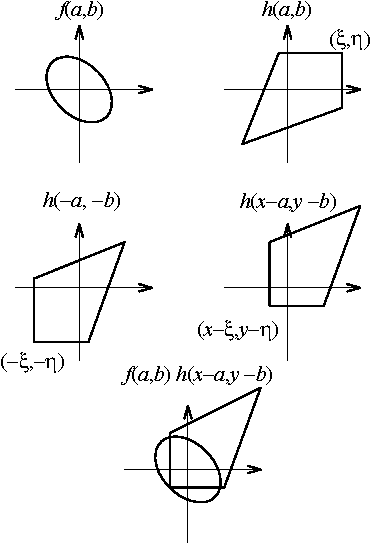
\includegraphics[scale=1.0]{01_signaly/images/img_1_1.pdf}
    \end{center}
    \caption{Průběh výpočtu konvoluce.}
    \label{img:1_1}
\end{figure}

Předpokládejme, že funkce \textit{h} je reprezentována maticí. Při praktických výpočtech často bývá funkce \textit{h} nenulová pouze v relativně malém počtu bodů (je-li to možné, pak takto funkci \textit{h} často záměrně volíme, aby časová složitost výpočtu konvoluce byla přijatelná). Při použití dosud uvedených vztahů jsou nenulové hodnoty většinou bohužel soustředěny do rohů matice, což komplikuje algoritmizaci a snižuje efektivnost výpočtu. V uvedeném případě je proto užitečné členy v matici reprezentující funkci \textit{h} přeskládat a odpovídajícím způsobem modifikovat vztahy pro výpočet konvoluce. Předpokládejme pro jednoduchost, že hodnoty \textit{M},\textit{N} jsou liché a položme \textit{P}=(\textit{M}$-$1)/2, \textit{Q}=(\textit{N}$-$1)/2. Zaveďme funkci $\tilde{h}$, která je definována nad oblastí $\{(m, n) | m = -P, -P+1, \dots, P$; $n = -Q, -Q+1, \dots, Q\}$, pomocí vztahu

\begin{equation} \label{eq:1_64}
    \tilde{h}(m, n) = \left\{
    \begin{array}{cc}
    h(-m, -n), & m \leq 0, n \leq 0 \\
    h(M - m, -n), & m > 0, n \leq 0 \\
    h(-m, N - n), & m \leq 0, n > 0 \\
    h(M - m, N - n), & m > 0, n > 0
    \end{array}
    \right. .
\end{equation}

\noindent S~využitím funkce $\tilde{h}$ lze pak pro výpočet konvoluce použít modifikovaného vztahu

\begin{equation} \label{eq:1_65}
    h(m, n) \ast f(m, n) = \frac{1}{MN} \sum\limits_{r=-P}^{P} \sum\limits_{s=-Q}^{Q} \tilde{h}(r, s) f\left( m + r, n + s \right).
\end{equation}

Předpokládejme, že funkční hodnoty $\tilde{h}(m,n)$ jsou nenulové pouze nad oblastí \{(\textit{m},\textit{n}) \textbar  \textit{m} = $-$\textit{R}, \dots, \textit{R}; \textit{n}= $-$\textit{S}, \dots, \textit{S}\}, kde \textit{R}$<$\textit{P}, \textit{S}$<$\textit{Q}. Ve vztahu \eqref{eq:1_65} pak stačí sčítat v~mezích $-$\textit{R}$\leq$\textit{r}$\leq$\textit{R}, $-$\textit{S}$\leq$\textit{s}$\leq$\textit{S} a k~praktické reprezentaci funkce $\tilde{h}$ na počítači stačí matice rozměru (2\textit{R}+1)$\times$(2\textit{S}+1) (pro tuto matici bývá často používáno termínu maska). Dále je zajímavé si povšimnout, že předpisem pro cyklickou konvoluci lze vypočítat též konvoluci lineární. Protože tato možnost má praktický význam, rozeberme ji podrobněji. Vyjděme ze vztahu \eqref{eq:1_65}, jímž se v praxi lineární konvoluce nejčastěji počítá. Uvažujme oblast $\tilde{\Omega} = \{(m, n) | m = 0, 1, \dots, M+R-1$; $n = 0, 1, \dots,  N+S-1\}$ a rozšiřme definici funkce \textit{f} na celou oblast $\tilde{\Omega}$ tak, že funkci \textit{f} položíme nad oblastí $\tilde{\Omega}\backslash\Omega$ rovnu nule. Nyní by již pro čtenáře mělo být snadným cvičením, aby ukázal, že lineární a cyklická konvoluce dají shodný výsledek.

